\section{Model Universes}

\begin{frame}{Model Universes}{Evolution of energy density}

	$$ P = w\epsilon; \hspace{1em} \dot\epsilon + 3\frac{\dot
	a}{a}(\epsilon + P) = 0 $$

By solving the state equation and the fluid equation alone, we can come up
with a relation
$$ \epsilon_i (a) = \epsilon_{i,0} a^{-3(1+w_i)}$$

The can be multiple explanations for why energy density decreases
\begin{itemize}[<+->]
	\item For matter, we have a $\epsilon \propto a^{-3}$, taking the value of
		$E_{mean}$ to be rest mass energy and constant we have that, the
		number density decreases cubically
	\item For radiation,$\epsilon \propto a^{-3}$ is due to the wavelength
		begin expanded (Emean reduces), but same the number density
		decreases.
	\item For Lambda matter, we have no dependence that means energy remains
		constant
\end{itemize}
\end{frame}


\begin{frame}{Model Universes}{Solved Friedmann equation}
Now if we use the relation we got by solving equation of state and fluid
equation in the friedmann equation we get:

$$ \dot a^2 = \frac{8\pi G}{3c^2} \sum \epsilon_i a^{-(1+3w_i)} -
\frac{\kappa c^2}{R_0} $$

Assuming the universe contains, Curvature, Matter, Radiation and Comsmological
Constant.

$$  \dot a^2 = \frac{8\pi G}{3c^2} ( \epsilon_\Lambda + \frac{\epsilon_r}{a^4} +  \frac{\epsilon_m}{a^3} ) -
\frac{\kappa c^2}{R_0}  $$

Using the relation in 4th chapter about curvature and using the definition of
$\epsilon_{c,0} = \frac{3c^2}{8\pi G}H_0^2 $ and $\frac{\kappa c^2}{R_0^2} = H_0^2(\Omega_0 - 1)$

$$ \frac{H^2}{H_0^2} = \frac{\Omega_{r,0}}{a^4} +
	\frac{\Omega_{m,0}}{a^3} + \Omega_{\Lambda,0} + \frac{1 - \Omega_{0}}{a^2} $$


\end{frame}

\begin{frame}{Model Universes}{General Procedure to solve the Model Universe}

\begin{itemize}[<+->]
	\item Using the friedman equation find out a relation between a(t) and
		t.
	\item Calculate z now using this relation.
	\item Calculate $d_p(t_o)$ interms of to and te. Use te = 0 to get
		horizon distance if exists.
	\item The get the $d_p(t_o)$ in terms of z instead of time.
	\item finally divide by 1+z to calculate $d_p(t_e)$.
\end{itemize}

The first part is usually the hardest part for more complex universes, but it
is simple for, empty universe (direct proportion), single flat component universe
(compare powers on the RHS and LHS).

by comparing powers we get:
$$ a(t) = \left(\frac{t}{t_0}\right)^{2/3+3w} $$

\end{frame}

\begin{frame}{Model Universes}{Empty Universes}
	When universe is empty (no energy density) the friedmann equation can be
	written as:
$$ \dot a^2 = - \kappa c^2 / R_0^2 $$

Values $\kappa = -1$, gives an interesting case where universe is expanding
linearly.

$$ \dot a^2 =  c^2 / R_0^2 $$
$$ a = \pm ct/R_0 $$

Finding $\frac{\dot a}{a} = H_0 = 1 / t_0$, which is original estimation of
hubble's constant that hubble performed.

The horizon distance is infinite and the proper distance in-terms of redshift comes out to be:
$$ d_p(t_0) = ct_0 \int^{t_o}_{t_e} \frac{dt}{a(t)} = \frac{c}{H_0} ln (1+z)$$

\end{frame}


\begin{frame}{Model Universes}{Single component}

A single component universe the friedmann equation can be written as:
$$ \dot a^2 = \frac{8\pi G\epsilon_0}{3c^2} a^{-(1+3w)} $$

Thus solving for relation between a and t.
$$ a(t) = \left( \frac{t}{t_0} \right)^{2/(3+3w)} $$

Using above relations we get some good usable relations like:
$$ d_p (t_0) = \frac{c}{H_0} \frac{2}{1+3w} [ 1 - (1+z)^{-(1+3w)/2} ] $$
$$ d_{Hor} (t_0) = \frac{c}{H_0} \frac{2}{1+3w} $$

\end{frame}


\begin{frame}{Model Universes}{Single component}

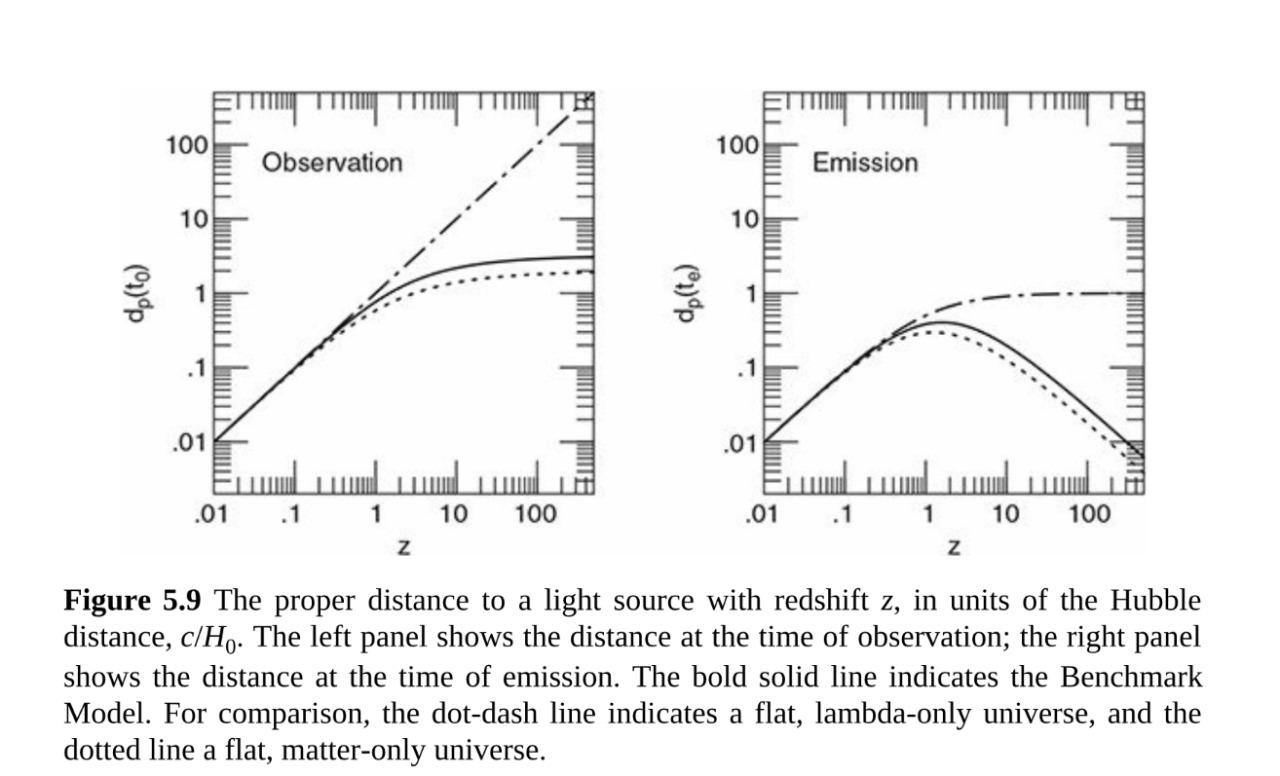
\includegraphics[width=2.2in]{3}
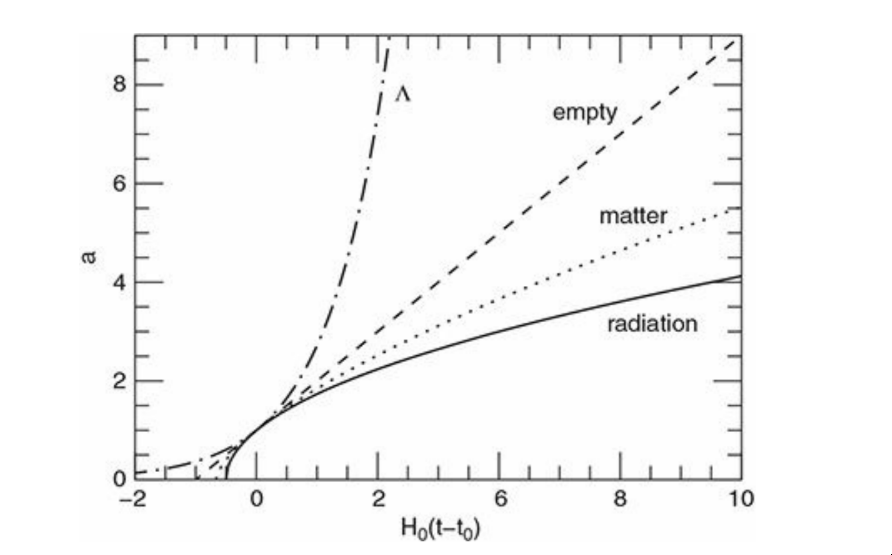
\includegraphics[width=2in]{6}

\end{frame}

\begin{frame}{Model Universes}{Multi component}

	It becomes difficult to integrate and find exact relations in multi
	component universe, hence most of the analysis is done frome the reduced
	version of friedmann equation itself.

	$$ \frac{H^2}{H_0^2} = \underbrace{\frac{\Omega_{r,0}}{a^4}}_{Radiation} +
	\underbrace{\frac{\Omega_{m,0}}{a^3}}_{Matter}
	+ \underbrace{\Omega_{\Lambda,0}}_{Cosmological constant} +
	\underbrace{\frac{1 - \Omega_{0}}{a^2}}_{Curvature} $$

	Where $\Omega_0 = \Omega_{r,0} + \Omega_{m,0} + \Omega_{\Lambda,0}$;
	and $\Omega_0 = 1 $ only if flat universe is   assumed

	If we vary the density parameters the values, we keep observing
	different dynamics in the universe
\end{frame}

\begin{frame}
	Example (matter + lambda + curvature):
	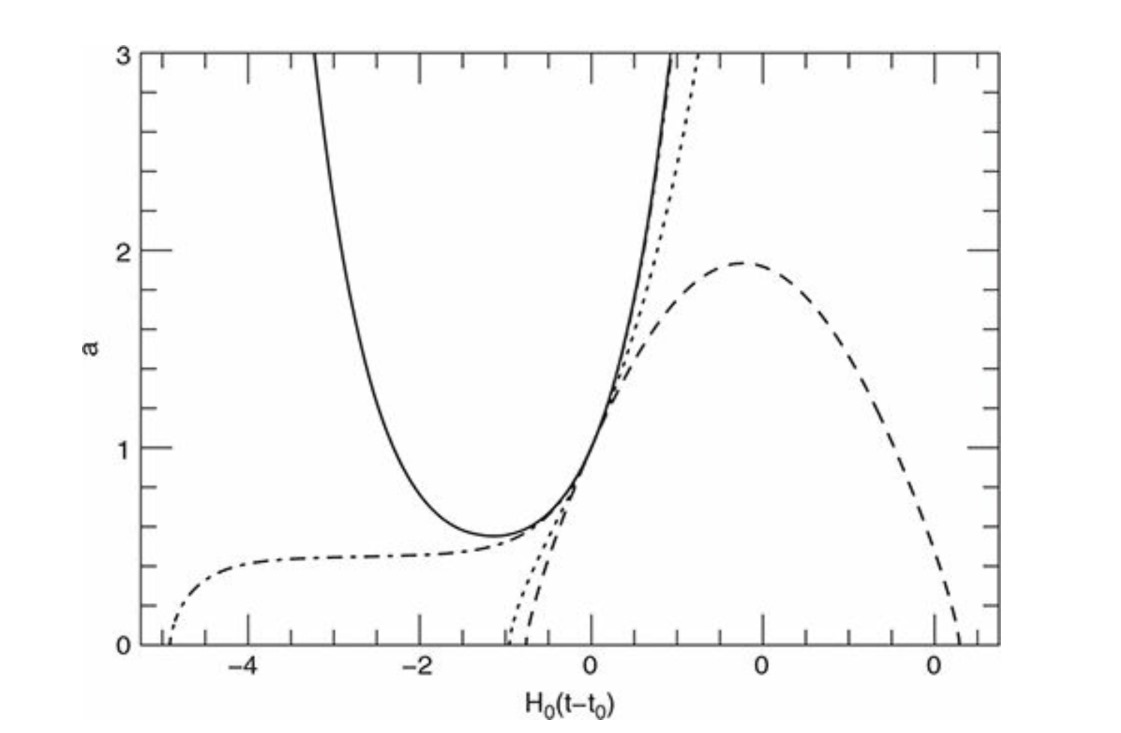
\includegraphics[width=\textwidth]{4}
\end{frame}

\begin{frame}{Model Universes}{Benchmark Universes}

	This is a good estimation to our current universe with the following
	parameters.

	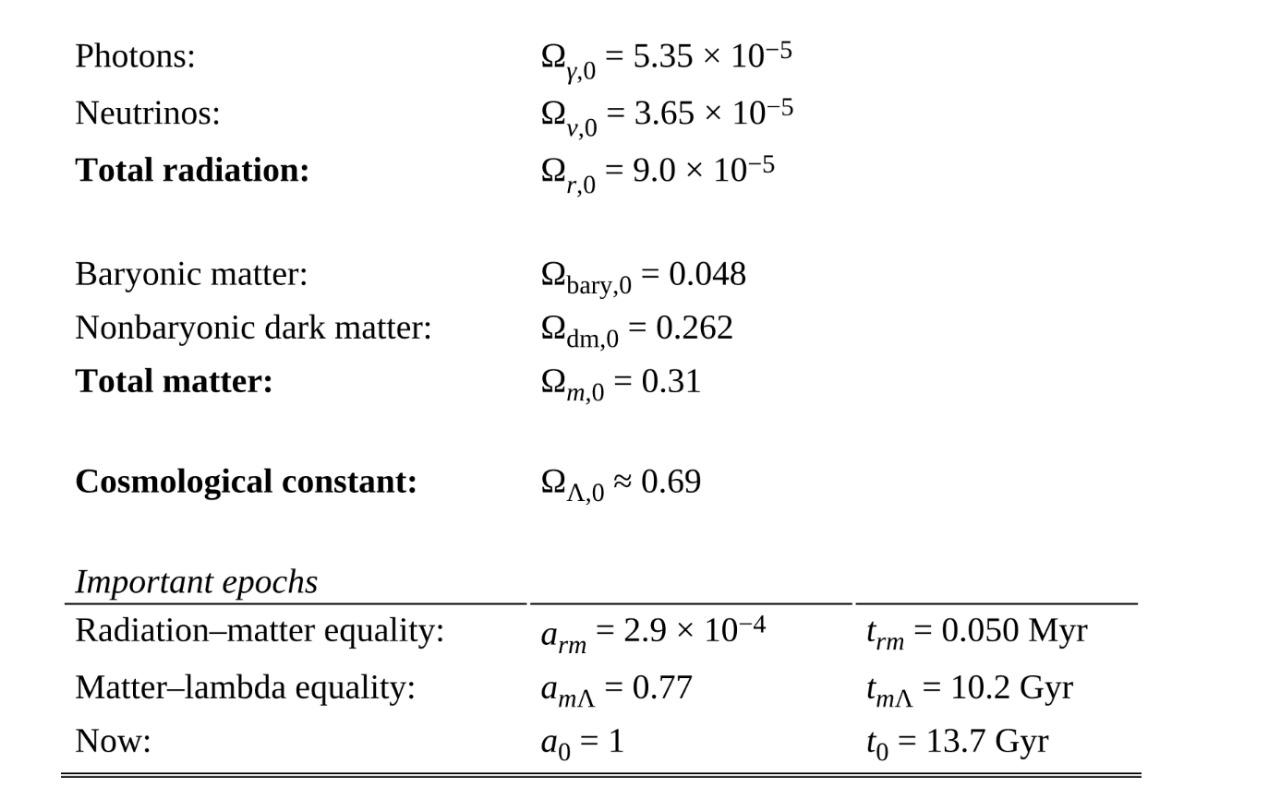
\includegraphics[width=0.9\textwidth]{5}
\end{frame}
